本节考虑如下的无约束优化问题:
\begin{equation}\label{ucp}
	\min\limits_{x\in\mathbb{R}^n} f(x),
\end{equation}
其中$f(x): \mathbb{R}^n\to\mathbb{R}$
\section{线搜索方法}
线搜索算法的数学表述为:给定当前点$x^k$,首先通过某种算法(稍后会涉及)选取\textbf{下降方向}$d^k$,确定\textbf{步长}$\alpha_k>0$,则下一步的迭代点可以写作
\begin{equation}\label{iter}
	x^{k+1} = x^k + \alpha_k d^k
\end{equation}
$d^k$是下降方向的要求为$(d^k)^T\nabla f(x^k)<0$,即要求了沿该方向函数值$f$会减小。线搜索回答了如何选择一个合适的步长$\alpha_k$.\par
实际上这是一个一维的优化问题,我们构造辅助函数
\begin{equation*}
	\phi(\alpha) = f(x^k+\alpha d^k)
\end{equation*}
显然,这是将$f(x)$限制在$\{x^k+\alpha d^k: \alpha > 0\}$一个一维区域上.线搜索的目的实际上是选取合适的$\alpha_k$使得$\phi(\alpha_k)$足够小,于是我们有两种想法:找到使函数值在该方向上的最小值或找到一个能够使函数值下降的步长(不需要下降到最小值),分别称为\textbf{精确线搜索算法}与\textbf{非精确线搜索算法}.
\subsection{精确线搜索算法}
正如上面所讨论的相同, 我们是求解如下的问题
\begin{equation*}
	\alpha_k = \arg \min\limits_{\alpha>0} \phi(\alpha),
\end{equation*}
即$\alpha_k$为最佳步长, 这实际上可能需要极大的计算量(针对光滑函数可以想象为求导函数的根,详情参见数值计算方法中求解非线性方程),所以我们在实际应用中很少使用这种方法,我们仅需要$\phi(\alpha_k)$满足一些不等式性质,这样产生的算法就是我们下面要介绍的\textbf{非精确搜索算法}
\subsection{Armijo准则}
首先,我们引入一个较为常用的线搜索准则,它保证了每一步迭代充分下降.
\begin{definition}[Armijo准则]
	设$d^k$为点$x^k$处的下降方向, 若
	\begin{equation*}\label{armijo}
		f(x^k+\alpha d^k)\leq f(x^k)+ c_1\alpha \nabla f(x^k)^Td^k,
	\end{equation*}
	则称步长$\alpha$满足\textbf{Armijo准则},其中$c_1\in (0, 1)$是一个预先给定的常数.
\end{definition}
Armijo准则的几何意义也是很明显的,参见下图
\begin{figure}[h!]
\caption{Armijo准则}
\centering
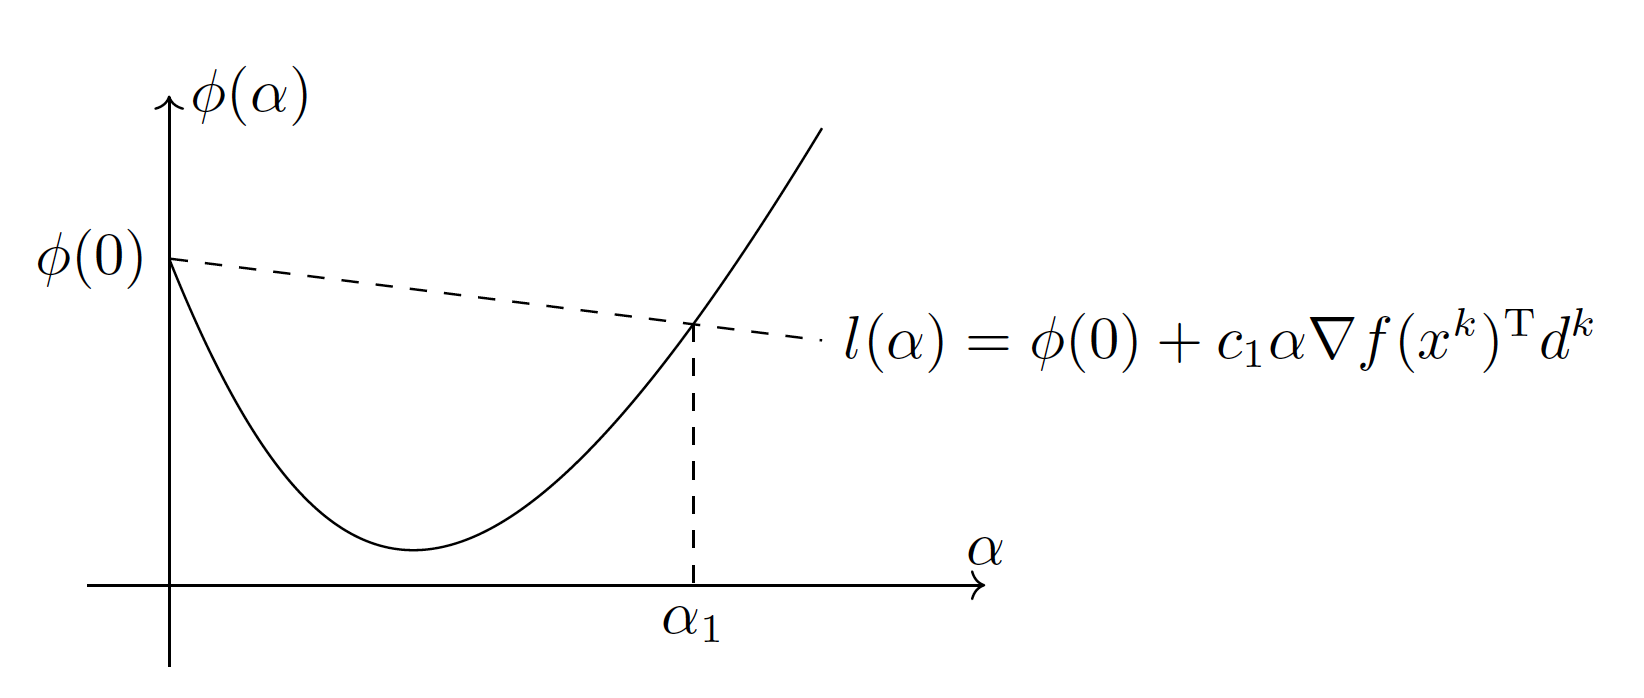
\includegraphics[width=0.8\textwidth]{img/armijo.png}
\end{figure}
它的含义是指点$(\alpha, \phi(\alpha))$必须在直线
\begin{equation*}
	l(\alpha) = \phi(0) +c_1\alpha \nabla f(x^k)^Td^k
\end{equation*}
的下方,由于$d^k$选取的是下降方向, 于是$\nabla f(x^k)^Td^k<0$,该直线的斜率一定为负.通常应用中取$c_1$足够小,这样使得Armijo条件非常容易满足,但是,如果选取的步长太小,那么迭代的点可能固定不变.\par
在实际使用过程中,我们常常将Armijo算法与\textbf{回退法}一同使用.给定初值$\hat{\alpha}$,回退法通过不断以指数方式缩小来试探步长,找到的第一个满足Armijo准则的点.
\begin{algorithm}[H]
%\footnotesize%字体大小
\caption{线搜索回退法}%首行显示算法名称
\begin{algorithmic}[1]%行编号,从Input, Output后面开始
%输入Input
\State 选择初始步长$\hat{\alpha}$,参数$\gamma, c\in (0, 1)$.初始化$\alpha\leftarrow \hat{\alpha}$.
\While{$f(x^k+\alpha d^k) > f(x^k)+ c_1\alpha \nabla f(x^k)^Td^k,$}
\State 令$\alpha \leftarrow \gamma \alpha$
\EndWhile
\State 输出$\hat{\alpha} = \alpha$
\end{algorithmic}  
\end{algorithm}
\subsection{Wolfe-Powell准则}
Wolfe-Powell准则也叫做Wolfe准则或Armijo-Wolfe准则.
\begin{definition}[Wolfe准则]
	设$d^k$是点$x^k$处的下降方向,若
	\begin{equation}\label{wolfe}
		\begin{split}
			&f(x^k+\alpha d^k)\leq f(x^k) + c_1\alpha \nabla f(x^k)^T d^k,\\
			&\nabla f(x^k + \alpha d^k)^T d^k \geq c_2 \nabla f(x^k)^Td^k,
		\end{split}
	\end{equation}
	则称步长$\alpha$满足\textbf{Wolfe准则},其中$c_1, c_2\in (0, 1)$为给定常数且有$c_1<c_2$.
\end{definition}
准则中第一个不等式即为Armijo准则,而第二个不等式为Wolfe准则的要求.注意到$\nabla f(x^k+\alpha d^k)^Td^k$恰好为$\phi(\alpha)$的导数,Wolfe准则实际要求$\phi(\alpha)$在$\alpha$处的切线斜率不能小于$\phi'(0)$的$c_2$倍.如图所示,在$[\alpha_1, \alpha_2]$中的点均满足Wolfe准则,并且在极小值点$\alpha^*$处有$\phi(\alpha^*) = \nabla f(x^k+\alpha^*d^k)^Td^k = 0$,于是$\alpha^*$永远满足第二个不等式, 只需选择较小的$c_1$满足第一个不等式即可。
\begin{figure}[h!]
\caption{Wolfe准则}
\centering
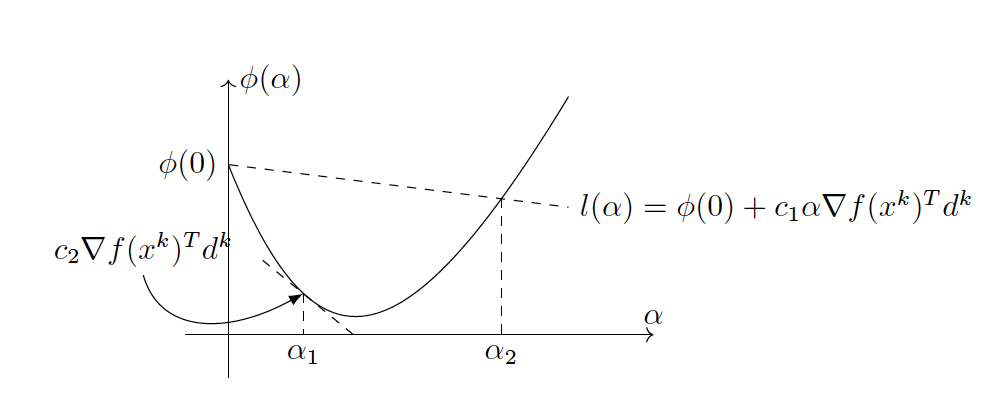
\includegraphics[width=0.8\textwidth]{img/wolfe.png}
\end{figure}
\subsection{线搜索法的收敛性分析}
\begin{theorem}[Zoutendijk]
	考虑一般的迭代格式\eqref{iter}.其中$d^k$是搜索发现, $\alpha_k$是步长, 且在迭代的过程中满足Wolfe准则. 假设目标函数$f$下有界、连续可微且梯度$\nabla f$ Lipschitz连续,即
	\begin{equation*}
		||\nabla f(x) - \nabla f(y)||\leq L||x-y||,\quad \forall x, y \in \mathbb{R}^n,
	\end{equation*}
	那么我们有
	\begin{equation*}
		\sum\limits_{k=0}^\infty \cos^2\theta_k ||\nabla f(x^k)||^2\leq +\infty
	\end{equation*}
	其中$\cos\theta_k$为负梯度$-\nabla f(x^k)$和下降方向$d^k$夹角的余弦, 即
	\begin{equation*}
		\cos\theta_k = \frac{-\nabla f(x^k)^Td^k}{||\nabla f(x^k)||||d^k||
}
	\end{equation*}
\end{theorem}
这个定理的证明是某老师喜欢考的,所以我们在此仔细加以讨论
\begin{proof}
	由Wolfe准则的第二个不等式,我们有
	\begin{equation*}
		(\nabla f(x^{k+1}) - \nabla f(x^k))^T d^k \geq (c_2 - 1)\nabla f(x^k)^Td^k.
	\end{equation*}
	有Cauchy-Schwarz不等式与Lipschitz条件
	\begin{equation*}
		\begin{split}
			(\nabla f(x^{k+1}) - \nabla f(x^k))^T d^k &\leq ||\nabla f(x^{k+1}) - \nabla f(x^k)||\ ||d^k||\\
			& \leq L||x^{k+1}-x^k||\ ||d^k||\\
			& \leq \alpha_k L ||d^k||^2.
		\end{split}
	\end{equation*}
	结合上面俩式,有
\begin{equation*}
	(c_2 - 1)\nabla f(x^k)^Td^k \leq \alpha_k L ||d^k||^2
\end{equation*}
即步长$\alpha_k$满足
\begin{equation*}
	\alpha_k \geq \frac{(c_2 - 1)\nabla f(x^k)^Td^k}{L ||d^k||^2}
\end{equation*}
将此式代入Wolfe准则的第一个不等式,得到
\begin{equation*}
	\begin{split}
		f(x^{k+1}) &\leq f(x^k) + c_1 \frac{(c_2 - 1)\nabla f(x^k)^Td^k}{L ||d^k||^2} \nabla f(x^k)^T d^k\\
		& = f(x^k)+\frac{c_1(c_2-1)}{L}\frac{(\nabla f(x^k)^T d^k)^2}{||d^k||^2}\\
		& = f(x^k)-\frac{c_1(1-c_2)}{L}\cos^2\theta_k ||\nabla f(x^k)||^2.
	\end{split}
\end{equation*}
这显然是一个递推的不等式, 右侧关于$k$递推(从$k$到$0$),得到
\begin{equation*}
	f(x^{k+1})\leq f(x^0)-\frac{c_1(1-c_2)}{L}\sum\limits_{j=0}^k\cos^2\theta_j ||\nabla f(x^j)||^2
\end{equation*}
由于$f$是下有界且下降的(Wolfe准则保证了严格下降性),同时由于$0<c_1<c_2<1$,有$c_1(1-x_2)>0$,于是我们得到了
\begin{equation*}
	\sum\limits_{j=0}^k\cos^2\theta_j ||\nabla f(x^j)||^2 < +\infty
\end{equation*}
令$k\to\infty$,得到我们所需要的
\begin{equation}\label{Zoutendijk}
	\sum\limits_{j=0}^\infty \cos^2\theta_j ||\nabla f(x^j)||^2 < +\infty
\end{equation}
\end{proof}
该定理指出了在满足Wolfe准则,对梯度Lipschitz连续且下有界的函数总能得到\eqref{Zoutendijk}条件成立.Zoutendijk定理实际上刻画了线搜索准则的性质, 配合一定的下降方向$d^k$选取方式, 我们能够得到线搜索最基本的收敛性.
\begin{theorem}[线搜索算法的收敛性]
	对于迭代格式\eqref{iter},设$\theta_k$为每一步迭代过程中下降方向$d^k$与负梯度方向$-\nabla f(x^k)$的夹角, 并且假设对于任意的$k$,都存在常数$\gamma$使得
	\begin{equation*}
		\theta_k < \frac{\pi}{2} - \gamma
	\end{equation*}
	严格成立,则在\eqref{Zoutendijk}条件成立的前提下, 我们能得到算法一定是收敛的,即
	\begin{equation*}
		\lim\limits_{k\to\infty} \nabla f(x^k) = 0.
	\end{equation*}
\end{theorem}
\begin{proof}
	直接证明较为困难,我们考虑反证法, 假设存在子列$\{k_l\}$和正常数$\delta > 0 $,使得结论不成立,即
	\begin{equation*}
		||\nabla f(x^{k_l})||\geq \delta,\quad l = 1, 2, \cdots,
	\end{equation*}
	根据$\theta_k$的假设,对任意$k$,有
	\begin{equation*}
		\cos\theta_k >\sin\gamma >0.
	\end{equation*}
	于是
	\begin{equation*}
		\begin{split}
			\sum\limits_{k=0}^\infty \cos^2\theta_k ||\nabla f(x^k)||^2  &\geq \sum\limits_{l=1}^\infty \cos^2\theta_{k_l} ||\nabla f(x^{k_l})||^2 \\
			&\geq \sum\limits_{l=1}^\infty (\sin^2\gamma)\cdot \delta^2\rightarrow +\infty
		\end{split}
	\end{equation*}
	这与\eqref{Zoutendijk}矛盾,因此一定有
	\begin{equation*}
		\lim\limits_{k\to\infty} \nabla f(x^k) = 0.
	\end{equation*}
\end{proof}
\begin{note}
	这个推论的几何意义是显然的, 如果下降方向$d^k$与梯度方向正交的话,根据Taylor公式的一阶近似, 函数值$f(x^k)$几乎不发生改变,因此我们在后面求解下降方向时,总是要求它与梯度的垂直方向的夹角有一定的下界, 这保证了我们在求解步长时的收敛性.
\end{note}
\section{梯度类算法}
梯度类算法实际上是采用了函数的一阶信息(即梯度Gradient),我们在这里只介绍梯度下降法与共轭梯度法.
\subsection{梯度下降法}
对于光滑函数$f(x)$,迭代至$x^k$处, 我们要选取一个合适的方向$d^k$作为下降方向.采用之前的记号$\phi(\alpha) = f(x^k +\alpha d^k)$,在$\alpha = 0$附近的一阶带Peano余项的Taylor展开
\begin{equation*}
	\phi(\alpha) = \phi(0) + \alpha \nabla f(x^k)^Td^k + \mathcal{O}(\alpha^2||d^k||^2),
\end{equation*}
由Cauchy-Schwarz不等式, 当$\alpha$足够小时, 选取$d^k = -\nabla f(x^k)$可使函数值下降最快, 于是我们有了梯度下降法的迭代格式
\begin{equation}\label{gd}
	x^{k+1}  = x^k - \alpha_k \nabla f(x^k).
\end{equation}
其中的$\alpha_k$既可以取为常数也可以采取一定算法取自适应步长.\par
在介绍具体的算法之前, 我们先分析该算法对对称正定的二次函数的收敛速度
\begin{theorem}
	考虑二次正定函数
	\begin{equation*}
		f(x) = \frac{1}{2}x^TAx - b^Tx,
	\end{equation*}
	其最优点$x^*$, 若使用梯度下降法\eqref{gd}并选取$\alpha_k$为精确线搜索的步长, 即
	\begin{equation*}
		\alpha_k = \frac{||\nabla f(x^k)||^2}{\nabla f(x^k)^T A \nabla f(x^k)},
	\end{equation*}
	那么梯度下降法是关于迭代点列$\{x^k\}$是Q-线性收敛(平方),即
	\begin{equation*}
		||x^{k+1}-x^*||_A^2 \leq \Big( \frac{\lambda_1-\lambda_n}{\lambda_1+\lambda_n}\Big)^2 ||x^{k}-x^*||_A^2
	\end{equation*}
	其中$\lambda_1,\lambda_n$分别为$A$的最大、最小特征值,$||x||_A\triangleq \sqrt{x^TAx}$为正定矩阵$A$诱导的范数.
\end{theorem}
\begin{note}
	我们可以推出如下的式子
	\begin{equation*}
		\frac{||x^{k+1}-x^*||_A}{||x^{k}-x^*||_A}\leq  \frac{|\lambda_1-\lambda_n|}{|\lambda_1+\lambda_n|}
	\end{equation*}
	取极限有,即在$||\cdot||_A$范数意义下, 迭代格式\eqref{gd}至少是线性收敛的.同时收敛比有一个上界
	\begin{equation*}
		\beta \leq \frac{|\lambda_1-\lambda_n|}{|\lambda_1+\lambda_n|}
	\end{equation*}
\end{note}
\begin{note}
	我们同时能发现, 该迭代方法的收敛速度与矩阵的谱(Spectrum)的分布有关,即特征值分布越密集,收敛越快.这个描述的几何意义是明显的, 当所有特征值都接近时,$\frac{|\lambda_1-\lambda_n|}{|\lambda_1+\lambda_n|}$的值达到最小值,即该二次函数的等高线近似为中心相同的一组圆. 
\end{note}
下面我们给出梯度下降法具体的算法,
\begin{algorithm}[H]
%\footnotesize%字体大小
\caption{梯度下降法}%首行显示算法名称
\begin{algorithmic}[1]%行编号,从Input, Output后面开始
%输入Input
\Require 控制误差$\varepsilon > 0$
\State 选择初始点$x^0$.初始化$k = 0$.
\While{$||\nabla f(x^k)|| \geq \varepsilon$}
\State 令下降方向$d^k\leftarrow -\nabla f(x^k)$
\State 做一维搜索
\begin{equation*}
	\alpha_k = \arg\min_{\alpha\geq 0} f(x^k + \alpha d^k)
\end{equation*}
\State 令$x^{k+1}\leftarrow x^k + \alpha_k d^k$,$k\leftarrow k+1$
\EndWhile
\State 输出$x^* = x^k$
\end{algorithmic}  
\end{algorithm}
\begin{note}
	对于做精确一维搜索的对称正定二次函数, 迭代格式如下
	\begin{equation*}
		x^{k+1} = x^k - \frac{||\nabla f(x^k)||^2}{\nabla f(x^k)^T A \nabla f(x^k)} \nabla f(x^k)
	\end{equation*}
\end{note}
关于做精确一维搜索的梯度下降法, 两次搜索的方向是彼此正交的,即有如下的命题
\begin{proposition}
	设$\{d^k\}$是由做精确一维搜索的梯度下降法产生的方向向量序列, 则有
	\begin{equation*}
		\langle d^k, d^{k+1}\rangle = 0 
	\end{equation*}
	其中$\langle \cdot, \cdot \rangle$为向量内积.
\end{proposition}
\begin{proof}
	引入之前的记号,
	\begin{equation*}
		\phi(\alpha) = f(x^k + \alpha d^k)
	\end{equation*}
	由于做精确的一维搜索, 我们不妨假设$f$足够光滑, 同时注意到$\alpha$为最优步长,则有
	\begin{equation*}
		\phi'(\alpha) = \nabla f(x^k + \alpha d^k)^T d^k = 0
	\end{equation*}
	而$d^{k+1} = \nabla f(x^k + \alpha d^k)$为在$k+1$次迭代时的方向,于是我们得到了
	\begin{equation*}
		\langle d^k, d^{k+1}\rangle = 0 
	\end{equation*}
	正是我们需要的.
\end{proof}
\begin{note}
	由于梯度下降法的相邻两次搜索方向闭相交, 于是在接近最优解的地方可能出现Zig-zag现象,即走“之”字型路线, 收敛性不够好.
\end{note}
\begin{figure}[h!]
\caption{Zig zag现象}
\centering
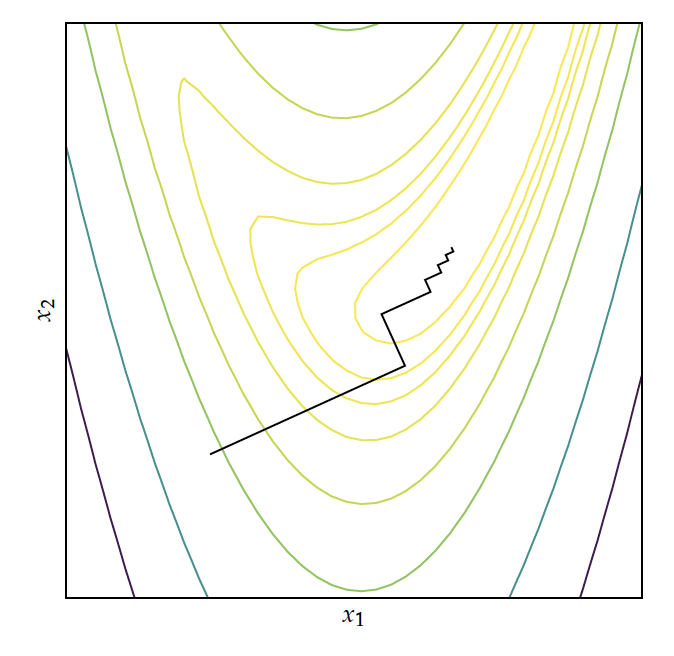
\includegraphics[width=0.6\textwidth]{img/zigzag.png}
\end{figure}
\section{共轭方向法}
在介绍共轭梯度法之前,我们先引入二次终止性的定义
\begin{definition}[二次终止性(Quadratic Termination)]
	如果一个算法对\textbf{二次正定函数}经过\textbf{有限次}迭代可以得到极小值点,这种算法具有\textbf{二次终止性}(Quadratic Termination).
\end{definition}
\begin{definition}[共轭向量]
	设$G$为$n$阶正定矩阵, $p^1, p^2,\cdots ,p^k$为$n$维向量组, 若
	\begin{equation*}
		{(p^i)}^TGp^j = 0,\quad i, j = 1,2,\cdots, k, i\neq j
	\end{equation*}
	则称向量组$p^1, p^2,\cdots ,p^k$关于$G$共轭
\end{definition}
\begin{note}
	实际上, 由矩阵特征向量(Eigenvector)的性质,我们容易有如下结果:
	\begin{enumerate}
		\item 共轭向量组线性无关,
		\item 共轭向量$p^1, p^2, \cdots, p^n$构成$\mathbb{R}^n$的一组基(思考为什么这里$k=n$),
		\item 求解共轭向量组实际上是求解矩阵特征向量.
	\end{enumerate}
\end{note}
待求解的问题为二次问题
\begin{equation}
	f(x) = \frac{1}{2}x^TGx+b^Tx+c
\end{equation}
进行$n$步搜索,由于$n$个共轭向量彼此线性无关,构成$\mathbb{R}^n$的一组基,故理论上经过$n$步就可以对二次正定函数得到最小值点.
\begin{algorithm}[H]
%\footnotesize%字体大小
\caption{共轭方向法}%首行显示算法名称
\begin{algorithmic}[1]%行编号,从Input, Output后面开始
%输入Input
\Require 控制误差$\varepsilon > 0$
\State 选择初始点$x^0$及初始下降方向$p^0$.初始化$k \leftarrow 0$.
\While{$||g^k||\geq \varepsilon$}
\State 做一维精确线搜索,确定步长
\begin{equation*}
	\alpha_k = \arg\min\limits_{\alpha \geq 0} f(x^k+\alpha p^k)
\end{equation*}
\State 令$x^{k+1}\leftarrow x^k + \alpha_k d^k$,$k\leftarrow k+1$
\State 取共轭方向$p^{k+1}$,使得
\begin{equation*}
	p^{k+1}Gp^i = 0,\quad i = 1, 2, \cdots, k.
\end{equation*}
\EndWhile
\State 输出$x^* = x^k$
\end{algorithmic}  
\end{algorithm}
下面给出求共轭方向的算法,类似Gram-Schimdt正交化方法, 记
\begin{equation*}
	\langle a, b\rangle_G = a^T G b
\end{equation*}
为正定矩阵$G$诱导出的内积, 容易验证其满足内积的定义(实际上就是将度量矩阵由$I$换为了对称正定矩阵$G$).
\begin{equation*}
	\begin{split}
		q^1 &= p^1\\
		q^2 &= p^2 - \frac{\langle p^2, q^1\rangle_G}{\langle p^1, q^1\rangle_G}q^1\\
		& \cdots \\
		q^n &= p^n -\sum \limits_{i=1}^{n-1}\frac{\langle p^n, q^i\rangle_G}{\langle p^i, q^i\rangle_G} q^i.\\
	\end{split}
\end{equation*}
下面介绍一种更简易的构造共轭方向的方法, 由于需要用到梯度,所以被称为共轭梯度法.
\section{共轭梯度法}
\begin{algorithm}[H]
%\footnotesize%字体大小
\caption{共轭梯度法}%首行显示算法名称
\begin{algorithmic}[1]%行编号,从Input, Output后面开始
%输入Input
\Require 控制误差$\varepsilon > 0$
\State 选择初始点$x^0$及初始下降方向$p^0$.初始化$k \leftarrow 0$.
\State $p_0 \leftarrow -g_0$
\State 
\begin{equation*}
	\beta_0\leftarrow \frac{(g^1)^TGp^0}{(p^0)^TGP^0}
\end{equation*}
\While{$||g^k||\geq \varepsilon$}
\State 令$p^{k+1} = -g^{k+1}+\beta_k p^k$,$k\leftarrow k+1$
\State $x^{k+1} \leftarrow x^k $
\State 
\begin{equation*}
	\beta_k \leftarrow \frac{(p^{k+1})^TGp^k}{(p^k)^TGp^k}
\end{equation*}
\EndWhile
\State 输出$x^* = x^k$
\end{algorithmic}  
\end{algorithm}

由于一般的函数求$G$(Hessian阵)计算量较大,于是我们给出几种不显含$G$的表达式.
\begin{equation*}
	\beta_{k-1} = \frac{(g^k)^TGp^{k-1}}{(p^{k-1})^TGp^{k-1}}
\end{equation*}
\subsection{Fletcher-Reeves公式}
由于
\begin{equation*}
	Gp^{k-1} = G\frac{1}{\alpha_{k-1}}(x^k-x^{k-1})=\frac{1}{\alpha_{k-1}}(g^k-g^{k-1})
\end{equation*}
于是
\begin{equation*}
	(g^k)^TGp^{k-1} = \frac{1}{\alpha_{k-1}}(g^k)^T(g^k-g^{k-1}) = {\alpha_{k-1}}(g^k)^T g^k
\end{equation*}
同时
\begin{equation*}
	(p^{k-1})^TGp^{k-1} = \frac{1}{\alpha_{k-1}}(-g^{k-1}+\beta_{k-2}p^{k-2})^T(g^k-g^{k-1}) = \frac{1}{\alpha_{k-1}}(g^{k-1})^Tg^{k-1}
\end{equation*}
故
\begin{equation*}
	\beta_{k-1} = \frac{(g^k)^Tg^k}{(g^{k-1})^Tg^{k-1}}
\end{equation*}
\begin{algorithm}[H]
%\footnotesize%字体大小
\caption{FR共轭梯度法}%首行显示算法名称
\begin{algorithmic}[1]%行编号,从Input, Output后面开始
%输入Input
\Require 控制误差$\varepsilon > 0$
\State 选择初始点$x^0$.初始化$k \leftarrow 0$.
\While{$||g^k||\geq \varepsilon$}
\State \begin{equation*}
	\beta_{k-1} = \begin{cases}
		\frac{(g^k)^Tg^k}{(g^{k-1})^Tg^{k-1}}, & k\geq 1\\
		0, &k=0.
	\end{cases}
\end{equation*}
\begin{equation*}
		p^k = -g^k + \beta_{k-1}p^{k-1}
\end{equation*}
\State 由一维搜索确定步长$\alpha_k$
\State 令$x^{k+1}\leftarrow x^k + \alpha_k p^k$,$k\leftarrow k+1$
\EndWhile
\State 输出$x^* = x^k$
\end{algorithmic}  
\end{algorithm}
\section{牛顿法}
本节我们讨论经典牛顿法,牛顿法属于二阶算法.对于二次连续可微函数$f(x)$,考虑其在$x^k$处的二阶Taylor展开
\begin{equation*}
	f(x^k + d^k) = f(x^k) + \nabla f(x^k)^Td^k+\frac{1}{2}(d^k)^T\nabla^2 f(x^k)d^k + \mathcal{o}(||d^k||^2)
\end{equation*}
将函数看做对$d^k$的极小化问题,并忽略高阶项,得到
\begin{equation*}
	h(d^k) = f(x^k) + \nabla f(x^k)^Td^k+\frac{1}{2}(d^k)^T\nabla^2 f(x^k)d^k
\end{equation*}
求导
\begin{equation*}
	\frac{\partial h}{\partial d^k} = \nabla f(x^k) + \nabla^2f(x^k)d^k = 0
\end{equation*}
得到$d^k$所满足的条件为
\begin{equation}\label{newtoneq}
	\nabla^2f(x^k)d^k = -\nabla f(x^k)
\end{equation}
上式\eqref{newtoneq}也被称为牛顿方程,容易得到当$\nabla^2f(x^k)$非奇异时,可以取$d^k = -\nabla^2f(x^k)^{-1}\nabla f(x^k)$.一般满足式\eqref{newtoneq}的方向也被称为\textbf{牛顿方向}.
经典牛顿法步长恒为$1$,因此其迭代格式为
\begin{equation*}
	x^{k+1} = x^k -\nabla^2f(x^k)^{-1}\nabla f(x^k).
\end{equation*}
如果步长可变, 则称之为阻尼牛顿法.
\section{拟牛顿法}
牛顿法在理论和实践上均有很好的效果,但由于其用到了二阶的Hessian阵,导致其对大规模问题的效果不是很好,于是我们猜想能否构造Hessian矩阵的近似矩阵,但任然保持一定的性质.我们接下来就将推导这些性质.
\subsection{割线方程}
回顾对牛顿法的推导过程,我们有
\begin{equation*}
	\nabla f(x) = \nabla f(x^{k+1}) +\nabla^2 f(x^{k+1})(x-x^{k+1}) + \mathcal{O}(||x-x^{k+1}||^2).
\end{equation*}
令$x=x^k, s^k = x^{k+1}-x^k, y^k = \nabla f(x^{k+1}) - \nabla f(x^k)$,并忽略高阶项,得到
\begin{equation*}
	\nabla^2f(x^{k+1})s^k = y^k
\end{equation*}
我们希望Hessian矩阵的近似矩阵$B^{k+1}$也满足同样的方程,即
\begin{equation}\label{quasinewton1}
	y^k = B^{k+1}s^k,
\end{equation}
或者其逆矩阵$H^{k+1}$近似满足
\begin{equation}\label{quasinewton2}
	s^k = H^{k+1}y^k,
\end{equation}
并称式\eqref{quasinewton1}与\eqref{quasinewton2}为\textbf{割线方程}.
\begin{algorithm}[H]
%\footnotesize%字体大小
\caption{拟牛顿法算法框架}%首行显示算法名称
\begin{algorithmic}[1]%行编号,从Input, Output后面开始
%输入Input
\Require 初始点$x^0\in\mathbb{R}^n$,初始矩阵$B^0\in\mathbb{R}^{n\times n}$(或$H^0$).\State 初始化$k \leftarrow 0$.
\While{未达到停机准则}
\State 计算方向$d^k = -(B^k)^{-1}\nabla f(x^k)$或$d^k = -H^k\nabla f(x^k)$.
\State 通过线搜索找到合适不长$\alpha_k>0$,令$x^{k+1} \leftarrow x^k+\alpha_k d^k$
\State 更新Hessian矩阵的近似矩阵$B^{k+1}$或其逆$H^{k+1}$.
\State $k\leftarrow k+1$
\EndWhile
\end{algorithmic}  
\end{algorithm}
实际使用过程中找$H^k$更为常用,因为这种方法不需要求解线性方程组.\par
实际上课本中介绍的BFGS公式(秩二更新)是为了改进秩一更新的部分缺点而提出的,详情还是请大家参考文再文老师的教材,这里就不展开细说了.
\subsection{BFGS公式}
我们考虑对Hessian阵近似矩阵$B^k$的秩二更新,采用待定系数法来推导公式,设
\begin{equation}
	B^{k+1} = B^k + auu^T+bvv^T,
\end{equation}
其中$u, v\in\mathbb{R}^n$,$a, b\in \mathbb{R}$待定.根据割线方程\eqref{quasinewton1},
\begin{equation*}
	B^{k+1}s^k = (B^k + auu^T+bvv^T)s^k  y^k,
\end{equation*}
整理得到
\begin{equation*}
	(a\cdot u^Ts^k)u + (b\cdot v^Ts^k)v = y^k-B^ks^k.
\end{equation*}
通过选取$u$和$v$让上述等式成立即可,一个较为显然的选法为对应项分别相等,即
\begin{equation*}
	\begin{split}
		u = y^k,\quad &a\cdot u^Ts^k = 1,\\
		v = B^ks^k,\quad & b\cdot v^Ts^k = -1.
	\end{split}
\end{equation*}
因此得到更新方式
\begin{equation}
	B^{k+1} = B^k+\frac{y^k(y^k)^T}{(s^k)^Ty^k} - \frac{B^ks^k(B^ks^k)^T}{(s^k)^TB^ks^k}.
\end{equation}
即为BFGS公式,它是由Broyden,Fletcher,Goldfarb,Shanno 四人名字的首字母组成
\subsection{DFP公式}
在BFGS公式的推导过程中,如果利用割线方程\eqref{quasinewton2}来对$H^k$进行秩二修正,得到基于$H^k$的拟牛顿矩阵更新
\begin{equation}
	H^{k+1} = H^k-\frac{H^ky^k(H^ky^k)^T}{(y^k)^TH^ky^k}+\frac{s^k(s^k)^T}{(y^k)^Ts^k}.
\end{equation}
上式即为DFP公式,这种迭代格式首先由Davidon 发现,此后由Fletcher 以及Powell进一步发展,因此被称为DFP 公式.